\documentclass{article}
\usepackage{bm}
\usepackage{mathtools}
\usepackage{fancyhdr}
\usepackage{extramarks}
\usepackage{amsmath}
\usepackage{amsthm}
\usepackage{amsfonts}
\usepackage{tikz}
\usepackage{graphicx}
\usepackage[plain]{algorithm}
\usepackage{algpseudocode}
\usepackage{cancel}
\usepackage{color,soul}
\usepackage{sidecap}
\usepackage{scalefnt}
\usetikzlibrary{automata,positioning}
\newcommand\hlight[1]{\tikz[overlay, remember picture,baseline=-\the\dimexpr\fontdimen22\textfont2\relax]\node[rectangle,fill=blue!50,rounded corners,fill opacity = 0.2,draw,thick,text opacity =1] {$#1$};} 


%
% Basic Document Settings
%

\topmargin=-0.45in
\evensidemargin=0in
\oddsidemargin=0in
\textwidth=6.5in
\textheight=9.0in
\headsep=0.25in

\linespread{1.1}

\pagestyle{fancy}
\lhead{\hmwkAuthorName}
\chead{\hmwkClass\ (\hmwkClassInstructor): \hmwkTitle}
\rhead{\firstxmark}
\lfoot{\lastxmark}
\cfoot{\thepage}

\renewcommand\headrulewidth{0.4pt}
\renewcommand\footrulewidth{0.4pt}

\setlength\parindent{0pt}

%
% Create Problem Sections
%

\newcommand{\enterProblemHeader}[1]{
    \nobreak\extramarks{}{Problem \arabic{#1} continued on next page\ldots}\nobreak{}
    \nobreak\extramarks{Problem \arabic{#1} (continued)}{Problem \arabic{#1} continued on next page\ldots}\nobreak{}
}

\newcommand{\exitProblemHeader}[1]{
    \nobreak\extramarks{Problem \arabic{#1} (continued)}{Problem \arabic{#1} continued on next page\ldots}\nobreak{}
    \stepcounter{#1}
    \nobreak\extramarks{Problem \arabic{#1}}{}\nobreak{}
}

\newcounter{partCounter}

\newcommand{\hmwkTitle}{Homework 05}
\newcommand{\hmwkDueDate}{March 15, 2016}
\newcommand{\hmwkClass}{Support Vector Machines}
\newcommand{\hmwkClassInstructor}{Dr. Lutz Hamel}
\newcommand{\hmwkAuthorName}{Robert Brown}

%
% Title Page
%

\title{
    \vspace{2in}
    \textmd{\textbf{\hmwkClass}}\\
    \textmd{\textbf{\hmwkTitle}}\\
    \normalsize\vspace{0.1in}\small{Due\ \hmwkDueDate}\\
    \vspace{3in}
}

\author{\textbf{\hmwkAuthorName}}
\date{}

\renewcommand{\part}[1]{\textbf{\large Part \Alph{partCounter}}\stepcounter{partCounter}\\}

%
% Various Helper Commands
%

% Useful for algorithms
\newcommand{\alg}[1]{\textsc{\bfseries \footnotesize #1}}

% For derivatives
\newcommand{\deriv}[1]{\frac{\mathrm{d}}{\mathrm{d}x} (#1)}

% For partial derivatives
\newcommand{\pderiv}[2]{\frac{\partial}{\partial #1} (#2)}

% Integral dx
\newcommand{\dx}{\mathrm{d}x}

% Alias for the Solution section header
\newcommand{\solution}{\textbf{\large Solution}}

% Probability commands: Expectation, Variance, Covariance, Bias
\newcommand{\E}{\mathrm{E}}
\newcommand{\Var}{\mathrm{Var}}
\newcommand{\Cov}{\mathrm{Cov}}
\newcommand{\Bias}{\mathrm{Bias}}

\makeatletter
\DeclareRobustCommand{\pder}[1]{%
  \@ifnextchar\bgroup{\@pder{#1}}{\@pder{}{#1}}}
\newcommand{\@pder}[2]{\frac{\partial#1}{\partial#2}}
\makeatother
  


\begin{document}

\maketitle

\pagebreak

For the midterm assignment, I plan on doing multi-class classification of the chars74k dataset -- a character set collected from google street view which exhibits tremendous irregularity.
These irregularities include different fonts, colors, image sizes, and off-axis characters. For learning to be feasible on this dataset, it is neccesary to somehow normalize
all of these variable parameters. To do this, I converted the images to a binary color scheme using Otsu Thresholding (https://en.wikipedia.org/wiki/Otsu's\_method). From here,
it is neccesary to determine the character and background colors (black or white) and normalize them across all images. This was done by finding the most frequent value
(black or white) along the perimeter, and assuming that this is the background color. This can be easly inverted, forcing all images backgrounds black and characters white.
The last step of normalization is scaling the images to all be the same pixel count (20x20), thus building a uniform feature vector (n=400).\\






\begin{figure}[!htb]
\minipage{0.32\textwidth}
  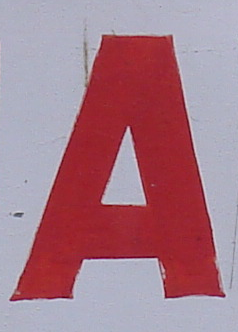
\includegraphics[width=\linewidth]{1122/original.png}
  \caption{Training image \#1122}\label{fig:awesome_image1}
\endminipage\hfill
\minipage{0.32\textwidth}
  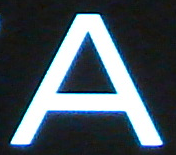
\includegraphics[width=\linewidth]{1653/original.png}
  \caption{Training image \#1653}\label{fig:awesome_image2}
\endminipage\hfill
\minipage{0.32\textwidth}%
  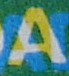
\includegraphics[width=\linewidth]{874/original.png}
  \caption{Training image \#874}\label{fig:awesome_image3}
\endminipage
\end{figure}

As this project is meant to be a binary classification problem, note that the largest single-character subset of the dataset could be taken and be used
to train a binary classification support vector machine. For an overview of the character distribution of the dataset, see the histogram below. 

\begin{figure}[!htb]
  \begin{center}
   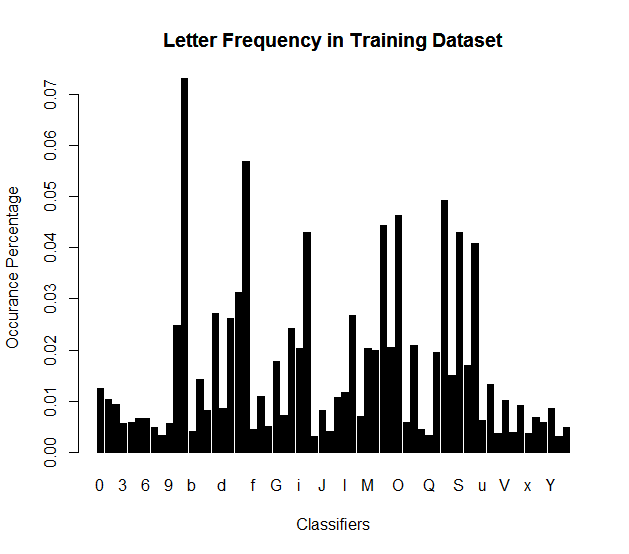
\includegraphics[width=7cm]{hist.png}
  \end{center}
\end{figure}

\begin{figure}[!htb]
\minipage{0.32\textwidth}
  
\includegraphics[width=\linewidth]{1122/processed.png}
  \caption{Normalized image \#1122}\label{fig:awesome_image1}
\endminipage\hfill
\minipage{0.32\textwidth}
  
\includegraphics[width=\linewidth]{1653/processed.png}
  \caption{Normalized image \$1653}\label{fig:awesome_image2}
\endminipage\hfill
\minipage{0.32\textwidth}%
  
\includegraphics[width=\linewidth]{874/processed.png}
  \caption{Normalized image \#874 }\label{fig:awesome_image3}
\endminipage
\end{figure}

Above, the normalized images can be seen. Below, the matrix representations of these images can be seen (in the same order as above). The feature vector is created by flattening these matricies into
one-dimensional structures. Lastly, note that for this type of high dimensional binary dataset, plots and summary statistics of the features are not particularly
useful as there are 400 features that can take only 0 or 1.

\begin{equation}
\begin{bmatrix}\begin{array}{ *{20}{c} }
0&0&0&0&0&0&0&0&0&0&0&0&0&0&0&0&0&0&0&0\\
0&0&0&0&0&0&0&0&0&0&0&0&0&0&0&0&0&0&0&0\\
0&0&0&0&0&0&0&0&0& \hlight{1} & \hlight{1} & \hlight{1} & \hlight{1} & \hlight{1} & \hlight{1} &0&0&0&0&0\\
0&0&0&0&0&0&0&0& \hlight{1} & \hlight{1} & \hlight{1} & \hlight{1} & \hlight{1} & \hlight{1} & \hlight{1} &0&0&0&0&0\\
0&0&0&0&0&0&0&0& \hlight{1} & \hlight{1} & \hlight{1} & \hlight{1} & \hlight{1} & \hlight{1} & \hlight{1} &0&0&0&0&0\\
0&0&0&0&0&0&0& \hlight{1} & \hlight{1} & \hlight{1} & \hlight{1} & \hlight{1} & \hlight{1} & \hlight{1} & \hlight{1} &0&0&0&0&0\\
0&0&0&0&0&0&0& \hlight{1} & \hlight{1} & \hlight{1} & \hlight{1} & \hlight{1} & \hlight{1} & \hlight{1} & \hlight{1} & \hlight{1} &0&0&0&0\\
0&0&0&0&0&0& \hlight{1} & \hlight{1} & \hlight{1} & \hlight{1} & \hlight{1} & \hlight{1} & \hlight{1} & \hlight{1} & \hlight{1} & \hlight{1} &0&0&0&0\\
0&0&0&0&0&0& \hlight{1} & \hlight{1} & \hlight{1} & \hlight{1} &0& \hlight{1} & \hlight{1} & \hlight{1} & \hlight{1} & \hlight{1} &0&0&0&0\\
0&0&0&0&0& \hlight{1} & \hlight{1} & \hlight{1} & \hlight{1} & \hlight{1} &0& \hlight{1} & \hlight{1} & \hlight{1} & \hlight{1} & \hlight{1} &0&0&0&0\\
0&0&0&0&0& \hlight{1} & \hlight{1} & \hlight{1} & \hlight{1} &0&0&0& \hlight{1} & \hlight{1} & \hlight{1} & \hlight{1} & \hlight{1} &0&0&0\\
0&0&0&0& \hlight{1} & \hlight{1} & \hlight{1} & \hlight{1} & \hlight{1} &0&0&0& \hlight{1} & \hlight{1} & \hlight{1} & \hlight{1} & \hlight{1} &0&0&0\\
0&0&0&0& \hlight{1} & \hlight{1} & \hlight{1} & \hlight{1} & \hlight{1} & \hlight{1} & \hlight{1} & \hlight{1} & \hlight{1} & \hlight{1} & \hlight{1} & \hlight{1} & \hlight{1} &0&0&0\\
0&0&0& \hlight{1} & \hlight{1} & \hlight{1} & \hlight{1} & \hlight{1} & \hlight{1} & \hlight{1} & \hlight{1} & \hlight{1} & \hlight{1} & \hlight{1} & \hlight{1} & \hlight{1} & \hlight{1} & \hlight{1} &0&0\\
0&0&0& \hlight{1} & \hlight{1} & \hlight{1} & \hlight{1} & \hlight{1} & \hlight{1} & \hlight{1} & \hlight{1} & \hlight{1} & \hlight{1} & \hlight{1} & \hlight{1} & \hlight{1} & \hlight{1} & \hlight{1} &0&0\\
0&0& \hlight{1} & \hlight{1} & \hlight{1} & \hlight{1} & \hlight{1} & \hlight{1} & \hlight{1} & \hlight{1} & \hlight{1} & \hlight{1} & \hlight{1} & \hlight{1} & \hlight{1} & \hlight{1} & \hlight{1} & \hlight{1} &0&0\\
0&0& \hlight{1} & \hlight{1} & \hlight{1} & \hlight{1} & \hlight{1} &0&0&0&0&0&0&0& \hlight{1} & \hlight{1} & \hlight{1} & \hlight{1} &0&0\\
0& \hlight{1} & \hlight{1} & \hlight{1} & \hlight{1} & \hlight{1} &0&0&0&0&0&0&0&0& \hlight{1} & \hlight{1} & \hlight{1} & \hlight{1} & \hlight{1} &0\\
0&0&0&0&0&0&0&0&0&0&0&0&0&0&0&0&0&0&0&0\\
0&0&0&0&0&0&0&0&0&0&0&0&0&0&0&0&0&0&0&0\\
\end{array}\end{bmatrix}
\end{equation}
\linebreak[20]

\begin{equation}
\begin{bmatrix}\begin{array}{ *{20}{c} }
0&0&0&0&0&0&0&0&0&0&0&0&0&0&0&0&0&0&0&0\\
0&0&0&0&0&0&0&0&0&0&0&0&0&0&0&0&0&0&0&0\\
0&0&0&0&0&0&0&0& \hlight{1} & \hlight{1} & \hlight{1} & \hlight{1} &0&0&0&0&0&0&0&0\\
0&0&0&0&0&0&0&0& \hlight{1} & \hlight{1} & \hlight{1} & \hlight{1} &0&0&0&0&0&0&0&0\\
0&0&0&0&0&0&0&0& \hlight{1} & \hlight{1} & \hlight{1} & \hlight{1} &0&0&0&0&0&0&0&0\\
0&0&0&0&0&0&0& \hlight{1} & \hlight{1} &0&0& \hlight{1} & \hlight{1} &0&0&0&0&0&0&0\\
0&0&0&0&0&0&0& \hlight{1} & \hlight{1} &0&0& \hlight{1} & \hlight{1} &0&0&0&0&0&0&0\\
0&0&0&0&0&0& \hlight{1} & \hlight{1} &0&0&0& \hlight{1} & \hlight{1} & \hlight{1} &0&0&0&0&0&0\\
0&0&0&0&0&0& \hlight{1} & \hlight{1} &0&0&0&0& \hlight{1} & \hlight{1} &0&0&0&0&0&0\\
0&0&0&0&0& \hlight{1} & \hlight{1} & \hlight{1} &0&0&0&0& \hlight{1} & \hlight{1} & \hlight{1} &0&0&0&0&0\\
0&0&0&0&0& \hlight{1} & \hlight{1} &0&0&0&0&0&0& \hlight{1} & \hlight{1} &0&0&0&0&0\\
0&0&0&0& \hlight{1} & \hlight{1} & \hlight{1} &0&0&0&0&0&0& \hlight{1} & \hlight{1} & \hlight{1} &0&0&0&0\\
0&0&0&0& \hlight{1} & \hlight{1} & \hlight{1} & \hlight{1} & \hlight{1} & \hlight{1} & \hlight{1} & \hlight{1} & \hlight{1} & \hlight{1} & \hlight{1} & \hlight{1} &0&0&0&0\\
0&0&0& \hlight{1} & \hlight{1} & \hlight{1} & \hlight{1} & \hlight{1} & \hlight{1} & \hlight{1} & \hlight{1} & \hlight{1} & \hlight{1} & \hlight{1} & \hlight{1} & \hlight{1} &0&0&0&0\\
0&0&0& \hlight{1} & \hlight{1} &0&0&0&0&0&0&0&0&0& \hlight{1} & \hlight{1} & \hlight{1} &0&0&0\\
0&0&0& \hlight{1} & \hlight{1} &0&0&0&0&0&0&0&0&0&0& \hlight{1} & \hlight{1} &0&0&0\\
0&0& \hlight{1} & \hlight{1} &0&0&0&0&0&0&0&0&0&0&0& \hlight{1} & \hlight{1} & \hlight{1} &0&0\\
0&0& \hlight{1} & \hlight{1} &0&0&0&0&0&0&0&0&0&0&0&0& \hlight{1} & \hlight{1} &0&0\\
0& \hlight{1} & \hlight{1} &0&0&0&0&0&0&0&0&0&0&0&0&0& \hlight{1} & \hlight{1} &0&0\\
0&0&0&0&0&0&0&0&0&0&0&0&0&0&0&0&0&0&0&0
\end{array}\end{bmatrix}\\
\end{equation}

\begin{equation}
\begin{bmatrix}\begin{array}{ *{20}{c} }
0&0&0&0&0&0&0&0&0&0&0&0&0&0&0&0&0&0&0&0\\
0&0&0&0&0&0&0&0&0&0&0&0&0&0&0&0&0&0&0&0\\
0&0&0&0&0&0&0&0& \hlight{1} & \hlight{1} & \hlight{1} & \hlight{1} &0&0&0&0&0&0&0&0\\
0&0&0&0&0&0&0&0& \hlight{1} & \hlight{1} & \hlight{1} & \hlight{1} & \hlight{1} &0&0&0&0&0&0&0\\
0&0&0&0&0&0&0& \hlight{1} & \hlight{1} & \hlight{1} & \hlight{1} & \hlight{1} & \hlight{1} &0&0&0&0&0&0&0\\
0&0&0&0&0&0& \hlight{1} & \hlight{1} & \hlight{1} & \hlight{1} & \hlight{1} & \hlight{1} & \hlight{1} & \hlight{1} &0&0&0&0&0&0\\
0&0&0&0&0&0& \hlight{1} & \hlight{1} & \hlight{1} & \hlight{1} &0& \hlight{1} & \hlight{1} & \hlight{1} &0&0&0&0&0&0\\
\hlight{1} &0&0&0&0&0& \hlight{1} & \hlight{1} & \hlight{1} &0&0&0& \hlight{1} & \hlight{1} & \hlight{1} &0&0&0&0&0\\
\hlight{1} &0&0&0&0& \hlight{1} & \hlight{1} & \hlight{1} & \hlight{1} &0&0&0& \hlight{1} & \hlight{1} & \hlight{1} & \hlight{1} &0&0&0&0\\
\hlight{1} &0&0&0&0& \hlight{1} & \hlight{1} & \hlight{1} & \hlight{1} &0&0&0& \hlight{1} & \hlight{1} & \hlight{1} & \hlight{1} &0&0&0&0\\
\hlight{1} &0&0&0&0& \hlight{1} & \hlight{1} & \hlight{1} &0&0&0&0&0& \hlight{1} & \hlight{1} & \hlight{1} & \hlight{1} &0&0&0\\
\hlight{1} &0&0&0& \hlight{1} & \hlight{1} & \hlight{1} & \hlight{1} & \hlight{1} & \hlight{1} & \hlight{1} &0&0& \hlight{1} & \hlight{1} & \hlight{1} & \hlight{1} &0&0&0\\
\hlight{1} &0&0&0& \hlight{1} & \hlight{1} & \hlight{1} & \hlight{1} & \hlight{1} & \hlight{1} & \hlight{1} & \hlight{1} & \hlight{1} & \hlight{1} & \hlight{1} & \hlight{1} & \hlight{1} & \hlight{1} &0&0\\
\hlight{1} &0&0& \hlight{1} & \hlight{1} & \hlight{1} & \hlight{1} & \hlight{1} & \hlight{1} & \hlight{1} & \hlight{1} & \hlight{1} &0& \hlight{1} & \hlight{1} & \hlight{1} & \hlight{1} & \hlight{1} &0&0\\
0&0&0& \hlight{1} & \hlight{1} & \hlight{1} & \hlight{1} &0&0&0&0&0&0&0& \hlight{1} & \hlight{1} & \hlight{1} & \hlight{1} &0&0\\
0&0& \hlight{1} & \hlight{1} & \hlight{1} & \hlight{1} & \hlight{1} &0&0&0&0&0&0&0&0& \hlight{1} & \hlight{1} & \hlight{1} & \hlight{1} &0\\
0&0& \hlight{1} & \hlight{1} & \hlight{1} & \hlight{1} &0&0&0&0&0&0&0&0&0&0& \hlight{1} & \hlight{1} & \hlight{1} &0\\
0&0&0&0&0&0&0&0&0&0&0&0&0&0&0&0&0&0&0&0\\
0&0&0&0&0&0&0&0&0&0&0&0&0&0&0&0&0&0&0&0\\
0&0&0&0&0&0&0&0&0&0&0&0&0&0&0&0&0&0&0&0\\
\end{array}\end{bmatrix}
\end{equation}

\end{document}

